\documentclass[12pt,a4paper,onecolumn]{article}

\usepackage[top=0.6in, left=0.6in,right=0.6in,bottom=0.6in]{geometry}
\usepackage{hyperref}
\usepackage{natbib}
\usepackage{listings}
\usepackage{color}
\usepackage{graphicx}
\usepackage{mathtools}

\author{Dionisio Perez-Mavrogenis}
\title{ELEC6032 Assignment}
 
\newcommand*\justify{%
  \fontdimen2\font=0.4em% interword space
  \fontdimen3\font=0.2em% interword stretch
  \fontdimen4\font=0.1em% interword shrink
  \fontdimen7\font=0.1em% extra space
  \hyphenchar\font=`\-% allowing hyphenation
}

\begin{document}
\maketitle

\section{Part 1}

The assigned elliptic curve E curve over the finite field $Z_{17}$ is 

$$ y^2 = x^3 + 4x + 3$$

together with the point at infinity, $O$.

\subsection{Find the order of your unique group}


\begin{table}[h]
\center
\caption{Field $E(Z_{17})$}
	\begin{tabular}{c c c c c c}
$(1,\pm5)$ & $(1,\pm12)$ & $(2,\pm6)$ & $(2,\pm11)$ & $(3,\pm5)$ & $(3,\pm12)$ \\
$(4,\pm7)$ & $(4,\pm10)$ & $(7,0)$    & $(11,\pm1)$ & $(11,\pm16)$ & $(13,\pm5)$ \\
$(13,\pm12)$ & $(14,\pm7)$ & $(14,\pm10)$ & $(15,\pm2)$ & $(15,\pm15)$ & $(16,\pm7)$ \\
$(16,\pm10)$ & $O$\\
	\end{tabular}
\label{table:points}
\end{table}

By the script given in Listing \ref{script_ecc} the cardinality of $E(Z_{17})$ is 38, the elements given in Table \ref{table:points}. Although one would expect that points should occur in pairs due to the symmetrical properties of elliptic curves, e.g. (15,2) and (15,-2), points with negative coordinates are not in $Z_{17}$, but there exist equivalent coordinates satisfying the equation, e.g. (15,15) instead of (15,-2).

\subsection{Is your group cyclic? Explain your answer}
Every elliptic curve over a field is an Abelian group under addition, with $O$ acting as the identity element. Every elliptic curve is a cyclic group or the product of two cyclic groups (i.e. has at most two generators), unless it is or prime order in which case it is cyclic \citep{website:cloudflare_primer} \citep{notes:ecc_notes}.


\subsection{Explain how elliptic curves can be used to construct secure ciphers}
The following follows closely \citep{book:ent}.

Two parties publicly agree on a prime number $p$, an elliptic curve $E$ over $Z/pZ$ (which is the field $Z_p$ of characteristic $p$) and a point $P\in E(Z_p)$. Then sender $A$ chooses a secret element $a$ and sends $aP$ to  $B$. $B$ also computes his secret element $b$ and sends $bP$ to $A$. They can both compute $abP$, which is their secret key. For an adversary to compute $n$ from $nP$ (or $m$) it would require solving the discrete logarithm problem for elliptic curves over a field.

The motivation to use elliptic curves is that the discrete logarithm problem is considered (mathematically) harder to solve for an elliptic curve over a field than it is for a finite field. Furthermore they are able to provide the same level of security as traditional PKI systems, with smaller key lengths (making them more attractive for using on smaller devices such as phones).\\

\subsection{Encrypt the following message using an appropriate elliptic curve cipher}
"A little knowledge is a dangerous thing"\\

\section{Part 2}
I believe this message is enciphered with a Vigenère cipher and the original text is:\\

\texttt{\justify the message starts here recently hardware trojans have attracted the attention of governments and researchers one of the main concerns is that integrated circuits in military or critical infrastructure applications could be maliciously manipulated during the manufacturing process which often takes place abroad however since there have been no reported hardware trojans in practice yet little is known about how such a trojan would look like and how hard to implement one in practice one example is dopant trojan this can be used to compromise the security of a meaningful real world target while avoiding detection by functional testing as well as trojan detection mechanisms such trojans can be used to establish a hidden side channel in an otherwise side channel resistant design this trojan does not change the logic value of any gate but instead changes only the power profile of two gates an evaluator who is not aware of the trojan cannot attack the trojan design using common side channel attacks the owner of the trojan however can use his knowledge of the trojan power model to establish a hidden side channel that reliably leaks out secret keys this is the end of the message}\\

This message looks like structured text and hence it might be encrypted with some mono-alphabetic substitution method. First I run it through a Caesar cracking tool with no meaningful results. Then I run it through \citep{tool:vigenere_cracker}, which yielded a meaningful message for key \texttt{xayxayxayxayxay}. However, by observing the key that \citep{tool:vigenere_cracker} derived one can see that it repeats itself and hence ,due to the nature of the cipher, the key could simply be \texttt{xay}. Furthermore Script \ref{code2} reports that the highest index of coincidence is found for a key length of 18, which is a multiple of 3.

In order to crack a Vigenère cipher, and due to this text's length which allows for meaningful statistical analysis, one can either employ the Kasisky test or the index of coincidence text to determine they key length. Once the key length has been determined one can treat the parts that correspond to each key-letter as simple mono-alphabetic substitution cipher and employ statistical methods.

\paragraph{Kasinsky Test} The Kasinski test is founded on the notion that texts which appear similar on the cipher-text will be the same plain-text that coincidentally was encrypted with the same key. The cryptanalyst looks for identical ciphertext bits that are at least three characters long and records the distance between those($\mathbf{\Delta} = {\Delta _1, \Delta _2, \dots , \Delta _n}$), as the distance is likely to be a multiple of the key-length (i.e. $\text{Length} = \text{gcd}(\mathbf{\Delta})$).

\paragraph{Index of Coincidence} The IoC method exploits the fact that letters in a language are not uniformly distributed in words and hence some letters will be more frequent than others. If the letter frequency was equal, then the probability of selecting the same random letter twice (in English) would be $\sum_{i=a}^{i=z}(1/26)^2 = 0.038$. Given the letter frequencies in English this probability is $\sum_{i=a}^{i=z}f_i ^2 = 0.067$, $f_i$ is the frequency of letter $i$. One can use this fact to test whether the plain-text was enciphered with a \textit{single-alphabet} cipher (e.g. Caesar) or not ,as the cipher-text's IoC would approximate that of the plain-text, i.e. 0.067/0.038 = 1.73. Once key-lengths that approach plain-text IoC are found they can be factored and a more systematic search can reveal likely key lengths.


\section{Part 3}
Here we knew that the second stage is an XOR cipher and the first two characters of the output, Hg. We get the key for the first two bytes by doing \texttt{Q" XOR Hg = 0x1945}(or 25 69 in decimal). A naive assumption worth investigating is to try this key for every two bytes of text, done by the script shown in Listing \ref{code1}. This produces the intermediate text shown bellow : \\

\texttt{\justify {Hgt ltsbuba pm dumt uy hgt lpyh wqpmpxbr sbr tdxyuct lvyhtqv pm hgtl sdd, xbobpib hp tctb hgt aqtshtyh lubry. Yxqtdv sbvpbt igp htddy vpx hgtv gsct hgt sbyitq uy npouba, lsr pq yulwdv luyhsotb. Hgtqt sqt lsbv hgubay hgsh lsot dumt ipqhg gpdruba pb hp sbr yscpxquba. Exh dumt uy xbwqtrukhsedt sbr it sqt pmhtb lvyhtquty tctb hp pxqytdcty. It hgubo yxkktyy, gswwubtyy, gtdwuba phgtqy, pq yxqwsyyuba pxqytdcty iudd lsot dumt ipqhg ducuba, exh it ksb sdisvy et iqpba pq mqxyhqshtr ev tctbhy. Hguy uy s qsbrpl wgqsyt. Wgudpypwgtqy gsct s dph hp ysv sepxh hgt csdxt pm sdd hgtyt hgubay, sbr s duhhdt dtyy hp ysv sepxh pbt pm hgt lpyh csdxsedt hgubay pm sdd: dpct. Yp it ksb et kdtsq tbpxag sepxh igsh uh ltsby mpq dumt hp gsct ltsbuba sbr csdxt, exh igtb it wxh rpib pxq wgudpypwgv eppoy sbr skhxsddv ath pb iuhg ducuba, ltsbuba sbr csdxt ksb et tdxyuct. Ducuba itdd uy lpqt sqh hgsb ykutbkt pq wgudpypwgv. Hgtqtmpqt,  hgt pbdv ytbyt it ksb lsot pm hgt urts hgsh dumt gsy ltsbuba uy hgsh hgtqt sqt yplt qtsypby hp duct qshgtq hgsb hp rut, sbr hgpyt qtsypby sqt hp et mpxbr ub hgt ducuba pm dumt uhytdm.}}\\

This text is sufficiently large to meaningful provide statistical information about its contents. More importantly, it looks like structured text, something which suggests that the first encryption stage might be a mono-alphabetic substitution. By using \citep{tool:design215} to get frequency overviews and perform substitutions, we get : \\

\texttt{\justify{the meaning of life is the most profound and elusive mystery of them all, unknown to even the greatest minds. surely anyone who tells you they have the answer is joking, mad or simply mistaken. there are many things that make life worth holding on to and savouring. but life is unpredicTable~and we are often mysteries even to ourselves. we think success, happiness, helping others, or surpassing ourselves will make life worth living, but we can always be wrong or frustrated by events. this is a random phrase. philosophers have a lot to say about the value of all these things, and a little less to say about one of the most valuable things of all: love. so we can be clear enough about what it means for life to have meaning and value, but when we put down our philosophy books and actually get on with living, meaning and value can be elusive. living well is more art than science or philosophy. therefore, the only sense we can make of the idea that life has meaning is that there are some reasons to live rather than to die, and those reasons are to be found in the living of life itself.}}\\

In order to understand the substitutions I looked for 1-letter words, which is most likely the article \texttt{a}. Having done that 2 and 3-letter words start appearing and analysing those is easier, as well as observing effects on longer words. Furthermore, the three-grams \texttt{SRB} , \texttt{SDD} and \texttt{NGT} are frequently found, and if we assume that \texttt{S} is really \texttt{a}, then \texttt{SRB} is \texttt{and} and \texttt{SDD} is \texttt{all}(that is the most likely scenario for these two words). Making these substitutions helped reveal more common words.

The next step that helped a lot was letter frequency, exploiTable~due to the texts length. The frequencies produced by \citep{tool:design215} are give in Table~\ref{freqs_q3}. Given the text's length it would be a fair to assume that some of the first letters are vowels, and hence substituting \texttt{T} for \texttt{e} gave further insight on the text. Now words with odd repetitions could be exploited, like \texttt{TCTB(eCeB)}, which contains an averagely common letter with another rare one. Furthermore, it would be safe to assume that \texttt{C} and \texttt{B} are both consonants. By trying words like \texttt{ever, even, eyes} revealed more information and the rest of the text was deciphered in a similar fashion.
 
\begin{table*}[t]
	\caption{\footnotesize Statistical information about the second-stage decrypted text. The top row statistics are for the English language, while the bottom refer to the text.}
	\label{freqs_q3}
	\resizebox{18cm}{!} {
	\begin{tabular}{c c c c c c c c c c c c c c c c c c c c c c c c c c}
E & T & A & O & I & N & S & H & R & D & L & C & U & M & W & F & G & Y & P & B & V & K & J & X & Q & Z\\
12.7 & 9.1 & 8.2 & 7.5 & 7.0 & 6.7 & 3.3 & 6.1 & 6.0 & 4.3 & 4.0 & 2.8 & 2.8 & 2.4 & 2.4 & 2.2 & 2.0 & 2.0 & 1.9 & 1.5 & 1.0 & 0.8 & 0.15 & 0.15 & 0.1 & 0.07\\
\hline
T & S & H & P & B & Y & U & D & G & Q & X & C & L & M & A & I & R & V & W & E & K & O & N & F & J & Z\\
113 & 73 & 72 & 68 & 67 & 65 & 56 & 52 & 49 & 41 & 28 & 21 & 21 & 21 & 20 & 19 & 19 & 17 & 15 & 14 & 11 & 8 & 1 & 0 & 0 & 0 \\
12.9 & 8.38 & 8.26 & 7.80 & 7.69 & 7.46 & 6.42 & 5.97 & 5.62 & 4.70 & 3.21 & 2.41 & 2.41 & 2.41 & 2.29 & 2.18 & 2.18 & 1.95 & 1.72 & 1.60 & 1.26 & 0.91 & 0.11 & 0 & 0 & 0\\
\hline
e & a & t & o & n & s & i & l & h & r & u & v & m & f & g & w & d & y & p & b & c & k & j \\
 
	\end{tabular}
}
\end{table*}


\section{Part 4}
In order to solve this part I used some online tools, as well as scripts that I wrote myself. In particular, I used \citep{tool:freq_analyzer} to perform frequency analysis and interactive letter substitutions, \citep{website:puzzle_info} to learn how the puzzles work and \citep{tool:design215} to search for words matching a given pattern.\\

Appendix \ref{headline_images} gives snapshots from the tool with the deciphered headlines and the letter frequencies. 
\subsection{Headline 1}
\paragraph{Solution} I believe this headline is the text: \texttt{ntsb urges new ways to combat rising runway incidents}.

One thing to note on this headline is that the first and last words ,\texttt{YNTS} and \texttt{CYOCMBYNT}, contain the same trigraph, \texttt{YNT}. Furthermore \texttt{CYOCMBYNT} contains two repeated letters and its ending must make sense in another word. The latter reasoning regarding word endings turned out to be misleading, as NTSB is an acronym for National Transportation Safety Board. 

After going through a couple of words produced with the pattern \texttt{---------/abcadebfg} by \citep{tool:design215}, the word \texttt{incident} seemed to make more sense in the context of a headline and how the substitutions affected other words. Substituting \texttt{inciMBnts} to the sentence, \texttt{HCTCYA} turned into \texttt{HisinA} and hence \texttt{A} is most likely \texttt{g}. After performing that substitution and \texttt{B} for \texttt{e} it appeared that \texttt{K} was most likely \texttt{w}. Now words like \texttt{QHges new wJVs} are appearing, suggesting text along the lines of \texttt{urges new ways} (\texttt{new} was a big give-away) and helping conclude that \texttt{R} is \texttt{o} after performing the substitutions so far.

After these previously mentioned steps, the rest of the text is fairly simple to deduce, contains no mistakes and makes sense in the context of a newspaper headline.

\subsection{Headline 2}
\paragraph{Result} I believe that this headline is the text: \texttt{dutch authorities closing in on human smuggling ring}.\\

To decipher this headline I firstly attempted to investigate the repetition of the letter \texttt{B} in \texttt{OAXBBJNHB} and the 9-letter words matching this pattern are shown in Table~\ref{words1}. Furthermore \texttt{OAXBBJNHB} ends in \texttt{HB}, as does \texttt{WNHB} and \texttt{YJVONHB}.

Additionally the two two-letter words \texttt{NH}
and \texttt{VH} are in the set shown in Table~\ref{words2}, both end with the letter \texttt{H} and should make sense syntactically and meaning-wise. The letter \texttt{H} in these words eliminates all words with \texttt{g, l} in their $8^{th}$ position from Table~\ref{words1}. Furthermore the word list in Table~\ref{words2} is further filtered by word likeliness, words whose second letter is not in any other word and by the possible $8^{th}$ position letters of Table~\ref{words1} words. This leaves a reduced list, shown in Table~\ref{words2}.

After using words ending in \texttt{s} and after using \texttt{crossties}, it seemed unlikely that \texttt{B} was \texttt{s} or that the word started with a \texttt{c}. Substituting \texttt{OAXBBJNHB} for the word \texttt{smuggling} some patterns in the words appeared, starting with the word \texttt{authorities} and from there on it was a case of the text making sense.

\begin{table}
	\center
	\caption{9-letter words with repeated 4th and 5th letters, ending on that letter as well.}
	\label{words1}

	\begin{tabular}{c c c c c c c}
	\hline
	blessings & blottiest & brattiest & brittlest & brummagem & chasseurs &  	chattiest\\
	coassumes & crossings & crosslets & crossties & crossways & draggling &  	dressings\\
	glassines & glissades & glossinas & gnattiest & grottiest & knottiest & plottiest\\
	plussages & pressings & reassigns & scheelite & smuggling & threesome &  trussings\\
	unseeable  \\
	\end{tabular}
\end{table}

\begin{table}
\caption{2-letter words and reduced list.}
\label{words2}

	\begin{tabular}{|c c c c c c c c c c c|}
	\hline
	ad & am & an & as & at & be & by & de & do & el & en \\
	go & he & id & if & in & is & it & ma & me & my & no \\
	nu & of & oh & on & or & pi & so & to & up & us & we \\
	\hline
	\end{tabular}
	\quad
	\begin{tabular}{|c c c c c c c|}
	\hline
	an & on & in & as & is & us & at\\
	it & be & he & me & we & by & my\\
	do & go & so & to & no & if & of\\
	\hline
	\end{tabular}
\end{table}

\subsection{Headline 3}
I believe this headline is the text : \texttt{dollar,euro outpace yen in choppy trading}.\\
How this headline was found follows later.
\subsection{Headline 4}
I believe this headline is the text : \texttt{ripken looking for quick return from disabled list}.\\
How this headline was found follows later.
\subsection{Headline 5}
I believe this headline is the text : \texttt{chrldless employees see discrimination in family friendly policies}.\\

The starting point for this headline was the ending of the word \texttt{TBDSPKTTY}, the word \texttt{YTT} and the ending of the word \texttt{HQUSESTYY}. The word \texttt{YTT} contains two very frequent letters, and one is a repetition. The letter \texttt{T} could be a vowel. The word \texttt{see} seemed like a very good candidate. Substituting \texttt{see} for \texttt{YTT} made the word \texttt{TBDSPKTTY} seem like \texttt{employees}, and after substitution, the first words started appearing.

The next stage of decryption was the word \texttt{JCBRSKJURTWESK}. The tool \citep{tool:design215} produces a list of words matching this pattern and after trial and error the most likely word is \texttt{discrimination}. 

After substitution of \texttt{discrimination}, the next word that seemed promising is \texttt{DPSRHRTY}, which most likely seems the be the word \texttt{policies}.

After performing all these substitutions, it is a matter of substituting the remaining letters and deciphering the message. The resulting message contains an error (one would expect ch\textit{i}ldless rather than ch\textit{r}ldless), but one would expect more errors to be in the sentence if the mapping was somehow forced to make the resulting plain-text.

\subsection{Discussion}
According to \citep{website:puzzle_info}, the first step to solving the puzzle is to build the mixed alphabet. Following the process described on the website (weaving of substitution chains of headlines 2 and 5 here, as I was unable to weave 2 and 3), the mixed alphabet produced was 
\texttt{girumbnwxachqlsykfjopdetvz}. To verify that this is correct, the mapping generated by sliding the alphabet against itself should decipher the solved headlines and produce meaningful text for the unsolved ones, which happens. The shift in the alphabet that solves each headline is $9, 5, 21, 7, 1$ and by stacking the resulting shifted-putative alphabets we can find the setting word, which I found to be \texttt{toady}. One can then reorder the alphabet so that \texttt{toady} is in the first column of the stacked alphabets and hence the shifted alphabet becomes  \texttt{sykfjopdetvzgirumbnwxachql}. Inputing that into the tool \citep{website:key_finder} yields the key \texttt{sycophant} and keyword square presented in Table~\ref{tab:ks}, indicating that the hat is of length 10.


\begin{table}
\center
\caption{The keyword square.}
\label{tab:ks}
	\begin{tabular}{c}
		\texttt{SYCOPHANTB}\\
		\texttt{DEFGIJKLMQ}\\
		\texttt{RUVWXZ}\\
	\end{tabular}
\end{table}


\bibliographystyle{plain}
\bibliography{crypto_report}

\pagebreak
\appendix
\section{Source code}

\textbf{Note} : The scripts in this section were produced by me in order to help me understand some concepts or aid my investigation. \\

\definecolor{gray}{rgb}{0.5,0.5,0.5}
\definecolor{bggray}{rgb}{0.9,0.9,0.9}
\definecolor{mygreen}{rgb}{0,0.5,0}

\lstdefinestyle{mypy}{
	backgroundcolor=\color{bggray},
	language=Python,
	basicstyle=\ttfamily,
  	captionpos=b,
	numbers=left, 
	keywordstyle=\color{blue}, 
	showspaces=false,
	commentstyle=\color{mygreen},
	numberstyle=\footnotesize\color{gray},
}

\lstinputlisting[caption=Code that performed the XOR operation with the key for question 3.,
				label=code1,
				style=mypy]
					{cw_files/question_3/question_3.py}
\lstinputlisting[caption=Code that perform shifting of the putative alphabet.,
				label=script_shift,
				style=mypy]
					{cw_files/question_4/headline.py}

\lstinputlisting[style=mypy, 
				caption=Code that iterates though the field $Z_{17}$ to check for solutions to elliptic curve E with equation $ y^2 \text{=} x^3 + 4x + 3 $.,
				label=script_ecc]
					{cw_files/question_1/ecc.py}

\pagebreak
\lstinputlisting[style=mypy,
				caption=Code that performs Index of Coincidence analysis.,
				label=code2]
					{cw_files/question_2/ioc.py}
\pagebreak										

\section{Headline Puzzle Substitutions}
\label{headline_images}

	\begin{figure*}[h]
		\center
		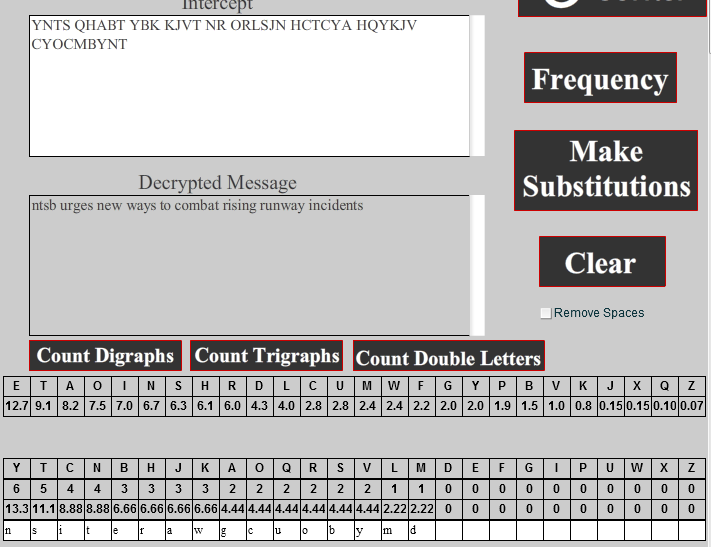
\includegraphics[scale=0.7]{cw_files/question_4/q1/q1_sol.png}
		\caption{Letter frequency analysis and mapping for headline 1.}
	\end{figure*}

	\begin{figure*}[h]
		\center
		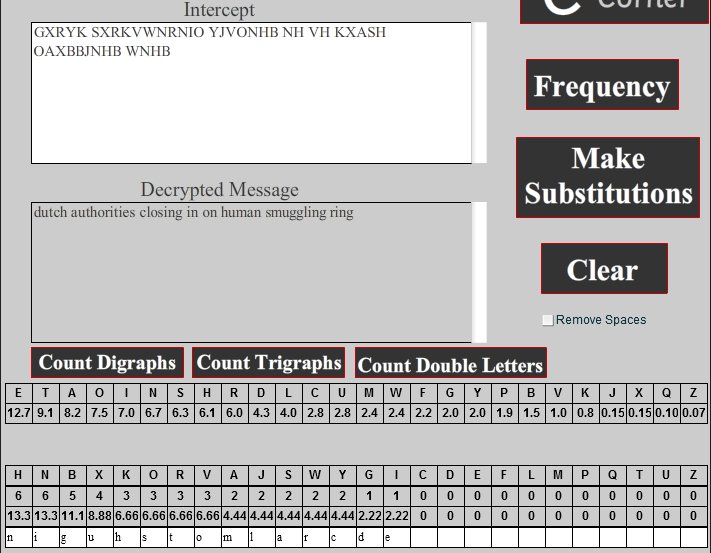
\includegraphics[scale=0.7]{cw_files/question_4/q2/Q2_sol.png}
		\caption{Letter frequency analysis and mapping for headline 2.}
	\end{figure*}
	
	\begin{figure*}[h]
		\center
		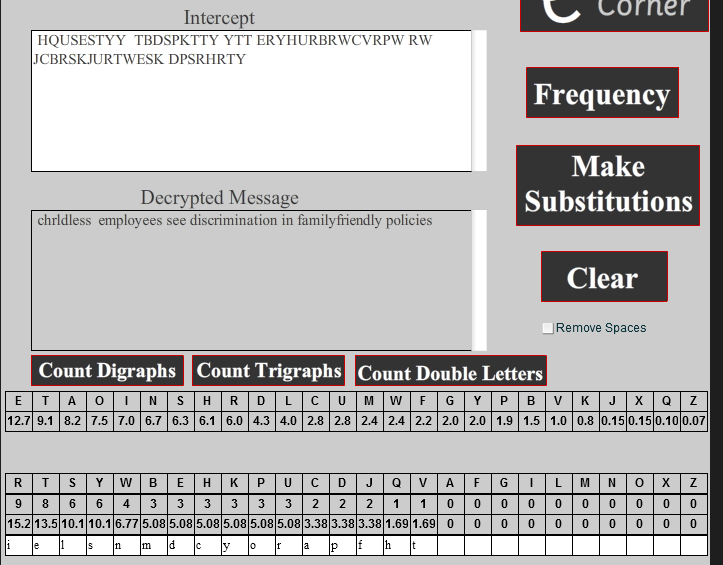
\includegraphics[scale=0.7]{cw_files/question_4/q5/puzzle_5.png}
		\caption{Letter frequency analysis and mapping for headline 5.}
	\end{figure*}

\end{document}
